\chapter{Specifikacija programske potpore}
		
	\section{Funkcionalni zahtjevi}
			
			
			\noindent \textbf{Dionici:}
			
			
			\begin{packed_enum}
				
				\item Korisnik
				\item Administrator				
				\item Vlasnik parkirališta(naručitelj)
				\item Razvojni tim
				
			\end{packed_enum}
			
			\noindent \textbf{Aktori i njihovi funkcionalni zahtjevi:}
			
			
			\begin{packed_enum}
				\item  \underbar{Neregistrirani korisnik (inicijator) može:}
				
				\begin{packed_enum}
					\item na karti pregledati lokacije parkirališta i tlocrt parkirališta
					\item stvoriti korisnički račun, tj. registrirati se za šta su mu potrebni korisničko ime, lozinka,  ime, prezime, slika osobne iskaznice, IBAN i email adresa 
				\end{packed_enum}
			
				\item  \underbar{Registrirani korisnik (sudionik) može:}
				
				\begin{packed_enum}
					\item prijaviti se u sustav koristeći korisničko ime i lozinku
					\item na karti odabrati adresu do koje želi doći
					\item na karti pregledati lokacije parkirališta, tlocrt parkirališta i dostupna parkirna mjesta
					\item rezervirati parkirno mjesto, termin i trajanje za koje je zainteresiran
					\item platiti rezervaciju parkinga 
				\end{packed_enum}
				
				\item  \underbar{Vlasnik parkinga (sudionik) može:}
				
				\begin{packed_enum}
					\item unijeti i mijenjati informacije o svom parkiralištu (naziv, opis, fotografija, cjenik)
					\item dodavati nova parkirna mjesta
					\item vidjeti statistiku zauzetosti parkirališta i parkirališnih mjesta kroz vrijeme
			 	\end{packed_enum}
			 	
				\item  \underbar{Administrator (sudionik) može:}
				
				\begin{packed_enum}
					\item pregledavati osobne podatke registriranih korisnika
					\item mijenjati osobne podatke registriranih korisnika
					\item potvrditi prijavu korisnicima koji se prijavljuju kao vlasnik parkinga
					
				\end{packed_enum}
			\end{packed_enum}
			\eject 
			
			
				
			\subsection{Obrasci uporabe}
				
				\subsubsection{Opis obrazaca uporabe}
					
					\noindent \underbar{\textbf{UC1 - registracija korisnika}}
					\begin{packed_item}
						
						\item \textbf{Glavni sudionik: }neregistrirani korisnik
						\item  \textbf{Cilj:} izraditi korisnički račun
						\item  \textbf{Sudionici:} baza podataka
						\item  \textbf{Preduvjet:} -
						\item  \textbf{Opis osnovnog tijeka:}
						
						\item[] \begin{packed_enum}
							
							\item korisnik odabire opciju za registraciju
							\item korisnik upisuje potrebne podatke
							\item u bazu podataka se upisuje novi korisnik
							\item web stranica se preusmjerava na stranicu za prijavu 
					
						\end{packed_enum}
						
						\item  \textbf{Opis mogućih odstupanja:}
						
						\item[] \begin{packed_item}
							
							\item[2.a] korisničko ime i/ili email su već zauzeti
							\item[] \begin{packed_enum}
								
								\item korisnik dobiva povratnu informaciju o specifičnoj greški i preusmjeren je nazad na stranicu za              registraciju
								
								
							\end{packed_enum}
							\item[2.b] upisana lozinka nije važeća(nema barem 8 znakova ili ne sadrži barem jedno slovo i brojku)
							\begin{packed_enum}
								
								\item korisnik dobiva povratnu informaciju o specifičnoj greški i preusmjeren je nazad na stranicu za              registraciju
								
								
							\end{packed_enum}
							
						\end{packed_item}
					\end{packed_item}
					
					\noindent \underbar{\textbf{UC2 -prijava korisnika}}
					\begin{packed_item}
						
						\item \textbf{Glavni sudionik: }registrirani korisnik
						\item  \textbf{Cilj:} prijava u korisnički račun
						\item  \textbf{Sudionici:} baza podataka
						\item  \textbf{Preduvjet:} prethodna registracija
						\item  \textbf{Opis osnovnog tijeka:}
						
						\item[] \begin{packed_enum}
							
							\item korisnik odabire opciju za prijavu
							\item korisnik upisuje svoje korisničko ime i lozinku
							\item korisnik je preusmjeren na početnu stranicu sa svim ovlastima prijavljenog korisnika
						
						\end{packed_enum}
						
						\item  \textbf{Opis mogućih odstupanja:}
						
						\item[] \begin{packed_item}
							
							\item[2.a] upisana kombinacija korisničkog imena i lozinke je neispravna
							\item[] \begin{packed_enum}
								
								\item korisnik je vraćen na stranicu za prijavu
								
							\end{packed_enum}
						
							
						\end{packed_item}
					\end{packed_item}
					
					\noindent \underbar{\textbf{UC3-promjena lozinke}}
					\begin{packed_item}
	
						\item \textbf{Glavni sudionik: }registrirani korisnik
						\item  \textbf{Cilj:} izmijeniti lozinku na već postojećem korisničkom računu
						\item  \textbf{Sudionici:} baza podataka
						\item  \textbf{Preduvjet:} prethodna registracija
						\item  \textbf{Opis osnovnog tijeka:}
						
						\item[] \begin{packed_enum}
	
							\item korisnik izabire opciju za mijenjanje lozinku
							\item korisnik upisuje email adresu na koju želi da mu se pošalje verifikacijski kod
							\item korisnik upisuje verifikacijski kod
							\item korisnik upisuje novu lozinku i potvrđuje ju ponovnim upisom
							\item korisnik je preusmjeren na stranicu za prijavu
						\end{packed_enum}
						
						\item  \textbf{Opis mogućih odstupanja:}
						
						\item[] \begin{packed_item}
	
							\item[3.a] upisani verifikacijski kod nije isti onom poslanom na email
							\item[] \begin{packed_enum}
								
								\item dolazi poruka o grešci i korisnik može opet upisati kod
								
							\end{packed_enum}
							\item[4.a] lozinke se ne poklapaju
							
							\begin{packed_enum}
								
								\item dolazi poruka o grešci i korisnik može opet upisati loznike
								
							\end{packed_enum}
							
							\item[4.b] upisana lozinka nije važeća(nema barem 8 znakova ili ne sadrži barem jedno slovo i brojku)
							
							\begin{packed_enum}
								
								\item dolazi poruka o grešci i korisnik može opet upisati loznike
								
							\end{packed_enum}
							
						\end{packed_item}
					\end{packed_item}
					
					\noindent \underbar{\textbf{UC4-odabir parkirališta}}
					\begin{packed_item}
						
						\item \textbf{Glavni sudionik: }prijavljeni korisnik
						\item  \textbf{Cilj:} izabrati parkiralište na kojem će kasnije rezervirati mjesto
						\item  \textbf{Sudionici:} sudionici
						\item  \textbf{Preduvjet:} prethodna prijava
						\item  \textbf{Opis osnovnog tijeka:}
						
						\item[] \begin{packed_enum}
							
							\item korisnik upisuje adresu do koje želi doći
							\item korisnik kliklne gumb za pretraživanje
							\item korisniku se na karti iscrta ruta do parkirališta koje je najbliže njegovom odredištu
						
						\end{packed_enum}
						
						 
					\end{packed_item}
					
					\noindent \underbar{\textbf{UC5.1 -rezervacija mjesta s uvjetom određenog mjesta}}
					\begin{packed_item}
						
						\item \textbf{Glavni sudionik: }prijavljeni korisnik
						\item  \textbf{Cilj:} rezervirati specifično parkirno mjesto
						\item  \textbf{Sudionici:} sudionici
						\item  \textbf{Preduvjet:} odabrano parkiralište
						\item  \textbf{Opis osnovnog tijeka:}
						
						\item[] \begin{packed_enum}
							
							\item korisnik klikne na ikonu parkirališta
							\item na karti parkirališta odabire mjesto za koje je zainteresiran
							\item u kalendaru izabire datum
							\item korisniku se prikazuju slobodni sati za odabrano mjesto i datum
							\item korisnik bira vremensko razdoblje
							\item korisnik potvrđuje rezervaciju
							\item web stranica se preusmjerava na stranicu za plaćanje
						\end{packed_enum}
						
						\item  \textbf{Opis mogućih odstupanja:}
						
						\item[] \begin{packed_item}
							
							\item[4.a] sva vremena za taj datum i mjesto su zauzeti
							\item[] \begin{packed_enum}
								
								\item korisnik sam mora odabrati neki drugi datum ili mjesto
								
							\end{packed_enum}
							
						\end{packed_item}
					\end{packed_item}
					
					\noindent \underbar{\textbf{UC5.2-rezervacija mjesta s uvjetom datuma}}
					\begin{packed_item}
						
						\item \textbf{Glavni sudionik: }prijavljeni korisnik
						\item  \textbf{Cilj:} rezervirati mjesto u specifičnom terminu
						\item  \textbf{Sudionici:} sudionici
						\item  \textbf{Preduvjet:} odabrano parkiralište
						\item  \textbf{Opis osnovnog tijeka:}
						
						\item[] \begin{packed_enum}
							
							\item korisnik klikne na ikonu parkirališta
							\item korisnik u kalendaru odabire datum i vrijeme početka parkiranja
							\item korisnik u kalendaru odabire datum i vrijeme završetka parkiranja 
							\item korisniku se prikažu dostupna mjesta za odabrani termin na karti parkirališta
							\item korisnik odabire mjesto na karti
							\item korisnik potvrđuje rezervaciju
							\item web stranica se preusmjerava na stranicu za plaćanje
						\end{packed_enum}
						
						\item  \textbf{Opis mogućih odstupanja:}
						
						\item[] \begin{packed_item}
							
							\item[4.a]niti jedno mjesto se ne prikazuje kao dostupno
							\item[] \begin{packed_enum}
								
								\item korisnik mora odabrati drugi termin
								
								
							\end{packed_enum}
							
							
						\end{packed_item}
					\end{packed_item}
					
					\noindent \underbar{\textbf{UC6.1-plaćanje prilikom dolaska}}
					\begin{packed_item}
						
						
						\item \textbf{Glavni sudionik: }prijavljeni korisnik
						\item  \textbf{Cilj:} plaćanje parkinga prilikom dolaska na lokaciju
						\item  \textbf{Sudionici:} baza podataka
						\item  \textbf{Preduvjet:} registracija korisnika
						\item  \textbf{Opis osnovnog tijeka:}
						
						\item[] \begin{packed_enum}
							
							\item 1. Korisnik dolazi rezervira parkirališno mjesto
							\item 2. Korisnik dolazi na lokaciju parkirališnog mjesta
							\item 3. Korisnik plaća rezervirano mjesto
						\end{packed_enum}
						
						\item  \textbf{Opis mogućih odstupanja:}
						
						\item[] \begin{packed_item}
							
							\item[2.a] opis mogućeg scenarija odstupanja u koraku 2
							\item[] \begin{packed_enum}
								
								\item opis rješenja mogućeg scenarija korak 1
								\item opis rješenja mogućeg scenarija korak 2
								
							\end{packed_enum}
							\item[2.b] opis mogućeg scenarija odstupanja u koraku 2
							\item[3.a] opis mogućeg scenarija odstupanja  u koraku 3
							
						\end{packed_item}
					\end{packed_item}
					
					\noindent \underbar{\textbf{UC6.2-plaćanje prilikom rezervacije}}
					\begin{packed_item}
						
						\item \textbf{Glavni sudionik: }prijavljeni korisnik
						\item  \textbf{Cilj:} plaćanje karticom prilikom rezervacije
						\item  \textbf{Sudionici:} baza podataka
						\item  \textbf{Preduvjet:} registracija korisnika
						\item  \textbf{Opis osnovnog tijeka:}
						
						\item[] \begin{packed_enum}
							
							\item 1. Korisnik odabire parkirališno mjesto i slobodan termin
							\item 2. Korisnik odabire mogućnost plaćanja karticom prilikom rezervacije
							\item 3. Korisnik unosi podatke s kartice
							\item 3. Nakon uspješnog plaćanja mjesto je rezervirano
						\end{packed_enum}
						
						\item  \textbf{Opis mogućih odstupanja:}
						
						\item[] \begin{packed_item}
							
							\item[2.a] odbijena kartica
							\item[] \begin{packed_enum}
								
								\item pojavljuje se poruka o nevaljanosti kartice
								\item opis rješenja mogućeg scenarija korak 2
								
							\end{packed_enum}
							\item[2.b] opis mogućeg scenarija odstupanja u koraku 2
							\item[3.a] opis mogućeg scenarija odstupanja  u koraku 3
							
						\end{packed_item}
					\end{packed_item}
					
					\noindent \underbar{\textbf{UC6.3-plaćanje sredstvima u novčaniku aplikacije}}
					\begin{packed_item}
						
						\item \textbf{Glavni sudionik: }prijavljeni korisnik
						\item  \textbf{Cilj:} plaćanje parkirnog mjesta sredstvima unutar aplikacije
						\item  \textbf{Sudionici:} baza podataka
						\item  \textbf{Preduvjet:} registracija korisnika, dodavanje novaca u novčanik
						\item  \textbf{Opis osnovnog tijeka:}
						
						\item[] \begin{packed_enum}
							
							\item 1. Korisnik sa svog računa uplaćuje željeni iznos u novčanik aplikacije
							\item 2. Korisnik prilikom rezervacije odabire način plaćanja sredstvima iz novčanika aplikacije
							\item 3. Nakon uspješnog plaćanja mjesto je rezervirano
						\end{packed_enum}
						
						\item  \textbf{Opis mogućih odstupanja:}
						
						\item[] \begin{packed_item}
							
							\item[2.a] nedovoljno sredstva u novčaniku
							\item[] \begin{packed_enum}
								
								\item pojavljuje se poruka o nedovoljnoj količini sredstava u novčaniku
								\item opis rješenja mogućeg scenarija korak 2
								
							\end{packed_enum}
							\item[2.b] opis mogućeg scenarija odstupanja u koraku 2
							\item[3.a] opis mogućeg scenarija odstupanja  u koraku 3
							
						\end{packed_item}
					\end{packed_item}
					
					\noindent \underbar{\textbf{UC7-dodavanje novaca u novčanik aplikacije}}
					\begin{packed_item}
						
						\item \textbf{Glavni sudionik: }prijavljeni korisnik
						\item  \textbf{Cilj:} korištenje sredstava novčanika aplikacije za plaćanje
						\item  \textbf{Sudionici:} baza podataka
						\item  \textbf{Preduvjet:} registracija korisnika
						\item  \textbf{Opis osnovnog tijeka:}
						
						\item[] \begin{packed_enum}
							
							\item 1. Korisnik odabire opciju za dodavanje sredstava u novčanik aplikacije
							\item 2. Korisnik upisuje podatke kartice te iznos koji želi uplatiti
							\item 3. Nakon uspješne uplate stanje u novčaniku aplikacije se ažurira
						\end{packed_enum}
						
						\item  \textbf{Opis mogućih odstupanja:}
						
						\item[] \begin{packed_item}
							
							\item[2.a] opis mogućeg scenarija odstupanja u koraku 2
							\item[] \begin{packed_enum}
								
								\item opis rješenja mogućeg scenarija korak 1
								\item opis rješenja mogućeg scenarija korak 2
								
							\end{packed_enum}
							\item[2.b] opis mogućeg scenarija odstupanja u koraku 2
							\item[3.a] opis mogućeg scenarija odstupanja  u koraku 3
							
						\end{packed_item}
					\end{packed_item}
					
					\noindent \underbar{\textbf{UC8-izmjena osobnih podataka korisnika}}
					\begin{packed_item}
						
						\item \textbf{Glavni sudionik: }administrator
						\item  \textbf{Cilj:} izmjena osobnih podataka postojećih korisnika
						\item  \textbf{Sudionici:} baza podataka
						\item  \textbf{Preduvjet:} registracija korisnika
						\item  \textbf{Opis osnovnog tijeka:}
						
						\item[] \begin{packed_enum}
							
							\item 1. Administrator odabire opciju pregled korisnika
							\item 2. Administrator otvara željeni profil
							\item 3. Administrator odabire opciju uredi
							\item 4. Administrator izmjenjuje podatke
							\item 5. Promjene se ažuriraju u bazi podataka
						\end{packed_enum}
						
						\item  \textbf{Opis mogućih odstupanja:}
						
						\item[] \begin{packed_item}
							
							\item[2.a] opis mogućeg scenarija odstupanja u koraku 2
							\item[] \begin{packed_enum}
								
								\item opis rješenja mogućeg scenarija korak 1
								\item opis rješenja mogućeg scenarija korak 2
								
							\end{packed_enum}
							\item[2.b] opis mogućeg scenarija odstupanja u koraku 2
							\item[3.a] opis mogućeg scenarija odstupanja  u koraku 3
							
						\end{packed_item}
					\end{packed_item}
					
					\noindent \underbar{\textbf{UC9-potvrđivanje prijave vlasniku}}
					\begin{packed_item}
						
						\item \textbf{Glavni sudionik: }administrator
						\item  \textbf{Cilj:} potvrda uspješne prijave voditelju
						\item  \textbf{Sudionici:} baza podataka
						\item  \textbf{Preduvjet:} registracija korisnika
						\item  \textbf{Opis osnovnog tijeka:}
						
						\item[] \begin{packed_enum}
							
							\item 1. Administrator odabire opciju pregled korisnika
							\item 2. Administrator otvara željeni profil
							\item 3. Administrator odabire opciju potvrdi voditelja
							\item 4. Promjene se ažuriraju u bazi podataka
						\end{packed_enum}
						
						\item  \textbf{Opis mogućih odstupanja:}
						
						\item[] \begin{packed_item}
							
							\item[2.a] opis mogućeg scenarija odstupanja u koraku 2
							\item[] \begin{packed_enum}
								
								\item opis rješenja mogućeg scenarija korak 1
								\item opis rješenja mogućeg scenarija korak 2
								
							\end{packed_enum}
							\item[2.b] opis mogućeg scenarija odstupanja u koraku 2
							\item[3.a] opis mogućeg scenarija odstupanja  u koraku 3
							
						\end{packed_item}
					\end{packed_item}
					
					\noindent \underbar{\textbf{UC10-brisanje korisnika}}
					\begin{packed_item}
						
						\item \textbf{Glavni sudionik: }administrator
						\item  \textbf{Cilj:}  izmjena osobnih podataka postojećih korisnika
						\item  \textbf{Sudionici:} baza podataka
						\item  \textbf{Preduvjet:} registracija korisnika
						\item  \textbf{Opis osnovnog tijeka:}
						
						\item[] \begin{packed_enum}
							
							\item 1. Administrator odabire opciju pregled korisnika
							\item 2. Administrator otvara željeni profil
							\item 3. Administrator odabire opciju uredi
							\item 4. Administrator izmjenjuje podatke
							\item 5. Promjene se ažuriraju u bazi podataka
						\end{packed_enum}
						
						\item  \textbf{Opis mogućih odstupanja:}
						
						\item[] \begin{packed_item}
							
							\item[2.a] opis mogućeg scenarija odstupanja u koraku 2
							\item[] \begin{packed_enum}
								
								\item opis rješenja mogućeg scenarija korak 1
								\item opis rješenja mogućeg scenarija korak 2
								
							\end{packed_enum}
							\item[2.b] opis mogućeg scenarija odstupanja u koraku 2
							\item[3.a] opis mogućeg scenarija odstupanja  u koraku 3
							
						\end{packed_item}
					\end{packed_item}
					
					\noindent \underbar{\textbf{UC11-unos podataka o parkiralištu}}
					\begin{packed_item}
						\item \textbf{Glavni sudionik: }voditelj parkinga
						\item  \textbf{Cilj:} unos podataka o parkirnom mjestu
						\item  \textbf{Sudionici:} baza podataka
						\item  \textbf{Preduvjet:} registracija korisnika, potvrda uloge voditelja
						\item  \textbf{Opis osnovnog tijeka:}
						
						\item[] \begin{packed_enum}
							
							\item 1. Voditelj otvara popis parkirališnih mjesta
							\item 2. Voditelj odabire željeno parkirališno mjesto
							\item 3. Voditelj odabire opciju uredi
							\item 4. Voditelj unosi naziv, opis, fotografiju, cijenu itd
							\item 5. Promjene se ažuriraju u bazi podataka
						\end{packed_enum}
						
						\item  \textbf{Opis mogućih odstupanja:}
						
						\item[] \begin{packed_item}
							
							\item[2.a] opis mogućeg scenarija odstupanja u koraku 2
							\item[] \begin{packed_enum}
								
								\item opis rješenja mogućeg scenarija korak 1
								\item opis rješenja mogućeg scenarija korak 2
								
							\end{packed_enum}
							\item[2.b] opis mogućeg scenarija odstupanja u koraku 2
							\item[3.a] opis mogućeg scenarija odstupanja  u koraku 3
							
						\end{packed_item}
					\end{packed_item}
					
					\noindent \underbar{\textbf{UC12-dodavanje dostupnosti parkirnog mjesta}}
					\begin{packed_item}
						
						\item \textbf{Glavni sudionik: }voditelj parkinga
						\item  \textbf{Cilj:} ucrtava dostupna parkirališna mjesta u kartu
						\item  \textbf{Sudionici:} baza podataka
						\item  \textbf{Preduvjet:} registracija korisnika, potvrda uloge voditelja
						\item  \textbf{Opis osnovnog tijeka:}
						
						\item[] \begin{packed_enum}
							
							\item 1. Voditelj otvara kartu parkirališnih mjesta
							\item 2. Voditelj odabire željeno parkirališno mjesto
							\item 3. Voditelj odabire opciju dostupno
							\item 4. Promjene se ažuriraju u bazi podataka
						\end{packed_enum}
						
						\item  \textbf{Opis mogućih odstupanja:}
						
						\item[] \begin{packed_item}
							
							\item[2.a] opis mogućeg scenarija odstupanja u koraku 2
							\item[] \begin{packed_enum}
								
								\item opis rješenja mogućeg scenarija korak 1
								\item opis rješenja mogućeg scenarija korak 2
								
							\end{packed_enum}
							\item[2.b] opis mogućeg scenarija odstupanja u koraku 2
							\item[3.a] opis mogućeg scenarija odstupanja  u koraku 3
							
						\end{packed_item}
					\end{packed_item}
					
					\noindent \underbar{\textbf{UC13-micanje dostupnosti parkirnog mjesta}}
					\begin{packed_item}
						
						\item \textbf{Glavni sudionik: }voditelj parkinga
						\item  \textbf{Cilj:} : ucrtava dostupna parkirališna mjesta u kartu
						\item  \textbf{Sudionici:} baza podataka
						\item  \textbf{Preduvjet:} registracija korisnika, potvrda uloge voditelja
						\item  \textbf{Opis osnovnog tijeka:}
						
						\item[] \begin{packed_enum}
							
							\item 1. Voditelj otvara kartu parkirališnih mjesta
							\item 2. Voditelj odabire željeno parkirališno mjesto
							\item 3. Voditelj odabire opciju nedostupno
							\item 4. Promjene se ažuriraju u bazi podataka
						\end{packed_enum}
						
						\item  \textbf{Opis mogućih odstupanja:}
						
						\item[] \begin{packed_item}
							
							\item[2.a] opis mogućeg scenarija odstupanja u koraku 2
							\item[] \begin{packed_enum}
								
								\item opis rješenja mogućeg scenarija korak 1
								\item opis rješenja mogućeg scenarija korak 2
								
							\end{packed_enum}
							\item[2.b] opis mogućeg scenarija odstupanja u koraku 2
							\item[3.a] opis mogućeg scenarija odstupanja  u koraku 3
							
						\end{packed_item}
					\end{packed_item}
					
					\noindent \underbar{\textbf{UC14-pregledavanje statistike za parkiralište}}
					\begin{packed_item}
						
						\item \textbf{Glavni sudionik: }voditelj parkinga
						\item  \textbf{Cilj:} pregled statistike zauzetosti parkirališnog mjesta
						\item  \textbf{Sudionici:} baza podataka
						\item  \textbf{Preduvjet:} registracija korisnika, potvrda uloge voditelja 
						\item  \textbf{Opis osnovnog tijeka:}
						
						\item[] \begin{packed_enum}
							
							\item 1. Voditelj otvara kartu parkirališnog mjesta
							\item 2. Voditelj odabire željeno parkirališno mjesto
							\item 3. Voditelj odabire opciju statistika
							\item 4. Prikazuje se statistika zauzetosti parkirališnog mjesta u obliku gafa
						\end{packed_enum}
						
						\item  \textbf{Opis mogućih odstupanja:}
						
						\item[] \begin{packed_item}
							
							\item[2.a] opis mogućeg scenarija odstupanja u koraku 2
							\item[] \begin{packed_enum}
								
								\item opis rješenja mogućeg scenarija korak 1
								\item opis rješenja mogućeg scenarija korak 2
								
							\end{packed_enum}
							\item[2.b] opis mogućeg scenarija odstupanja u koraku 2
							\item[3.a] opis mogućeg scenarija odstupanja  u koraku 3
							
						\end{packed_item}
					\end{packed_item}
					
					\noindent \underbar{\textbf{UC15 -pregled parkirališnih mjesta}}
					\begin{packed_item}
						
						\item \textbf{Glavni sudionik: }korisnik
						\item  \textbf{Cilj:} pregled parkirališnih mjesta i njihova dostupnost
						\item  \textbf{Sudionici:} baza podataka
						\item  \textbf{Preduvjet:} -
						\item  \textbf{Opis osnovnog tijeka:}
						
						\item[] \begin{packed_enum}
							
							\item 1. Korisnik odabire kartu parkirališta
							\item 2. Otvara se karta sa prikazom dostupnih mjestas
						\end{packed_enum}
						
						\item  \textbf{Opis mogućih odstupanja:}
						
						\item[] \begin{packed_item}
							
							\item[2.a] opis mogućeg scenarija odstupanja u koraku 2
							\item[] \begin{packed_enum}
								
								\item opis rješenja mogućeg scenarija korak 1
								\item opis rješenja mogućeg scenarija korak 2
								
							\end{packed_enum}
							\item[2.b] opis mogućeg scenarija odstupanja u koraku 2
							\item[3.a] opis mogućeg scenarija odstupanja  u koraku 3
							
						\end{packed_item}
					\end{packed_item}

				\section{Dijagram obrazaca uporabe} 
			
			{ Na slici je prikazan dijagram obrazaca uporabe točnije funkcionalnosti korisnika, registriranog korisnika, administratora te voditelja parkinga. }
			
			\begin{figure}[h]
				\centering
				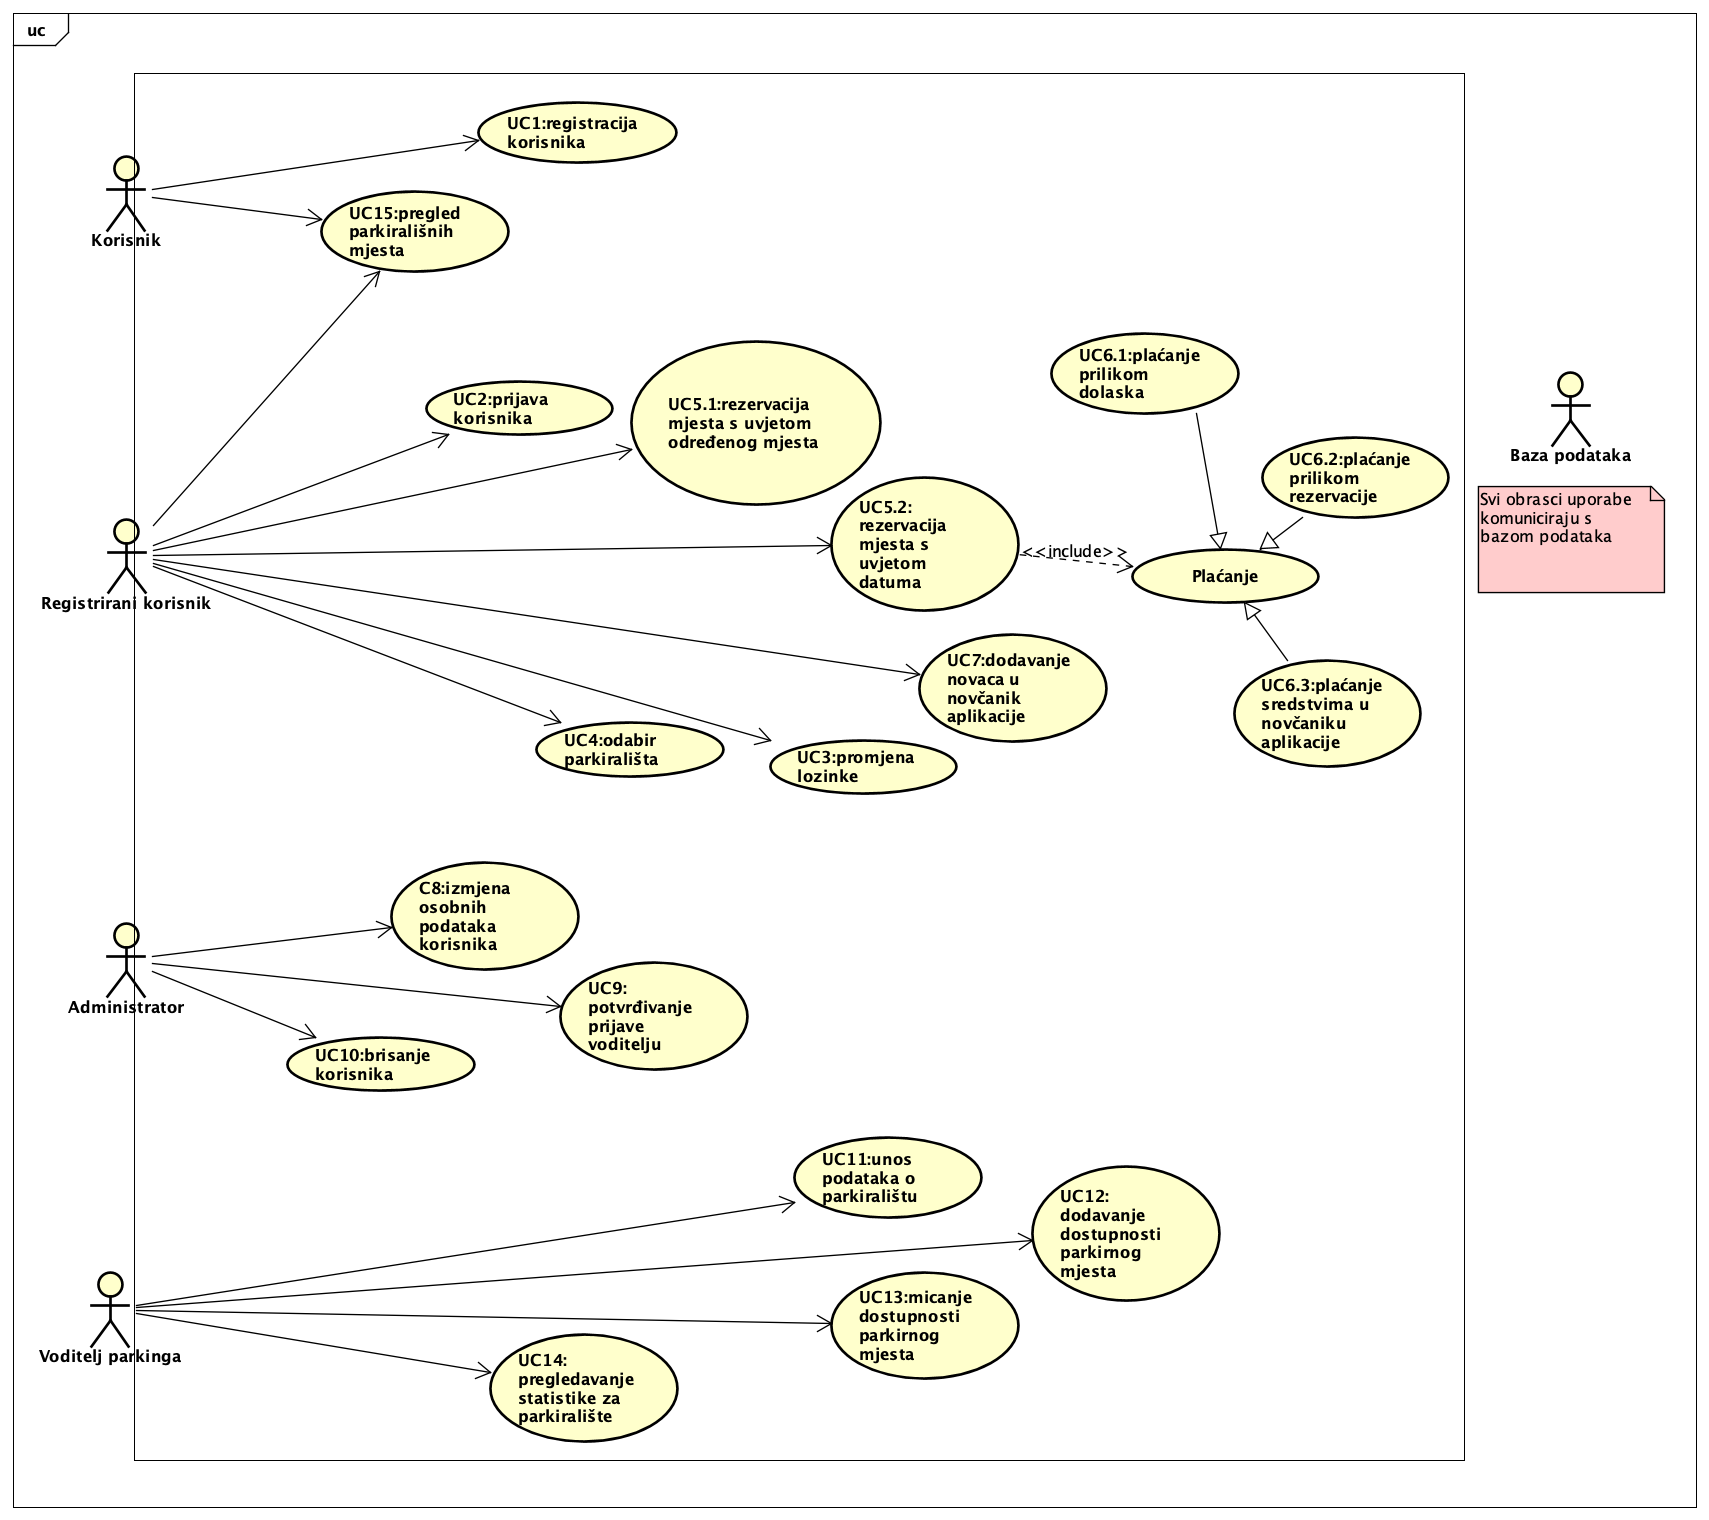
\includegraphics[width=\textwidth,keepaspectratio]{slike/spotPicker.png}
			\end{figure}
			\pagebreak
				

					
				\subsubsection{Dijagrami obrazaca uporabe}
					
					\textit{Prikazati odnos aktora i obrazaca uporabe odgovarajućim UML dijagramom. Nije nužno nacrtati sve na jednom dijagramu. Modelirati po razinama apstrakcije i skupovima srodnih funkcionalnosti.}
				\eject		
				
			\subsection{Sekvencijski dijagrami}
				
				 \textbf{\textit{Obrazac uporabe UC4 - Odabir parkirališta}}
				  
				
				 \textit{Klijent, nakon što pokrene aplikaciju, šalje zahtjev za pregled svih dostupnih parkirališta. Aplikacija, koristeći bazu podataka, dohvaća popis parkirališta te ih prikazuje korisniku. Nakon pregleda, klijent odabire specifično parkiralište koje ga zanima. Aplikacija zatim prikazuje dodatne informacije o odabranom parkiralištu, uključujući naziv, opis, fotografiju, cjenik i slobodna parkirališna mjesta. Dodatno, klijent može pregledati dostupna parkirališna mjesta na karti povezanoj s odabranim parkiralištem, a ovisno o odabiru, informacije o zauzetosti pojedinih mjesta}
				    
				       \begin{figure}[hbt!]
				    	   \centering
				    	   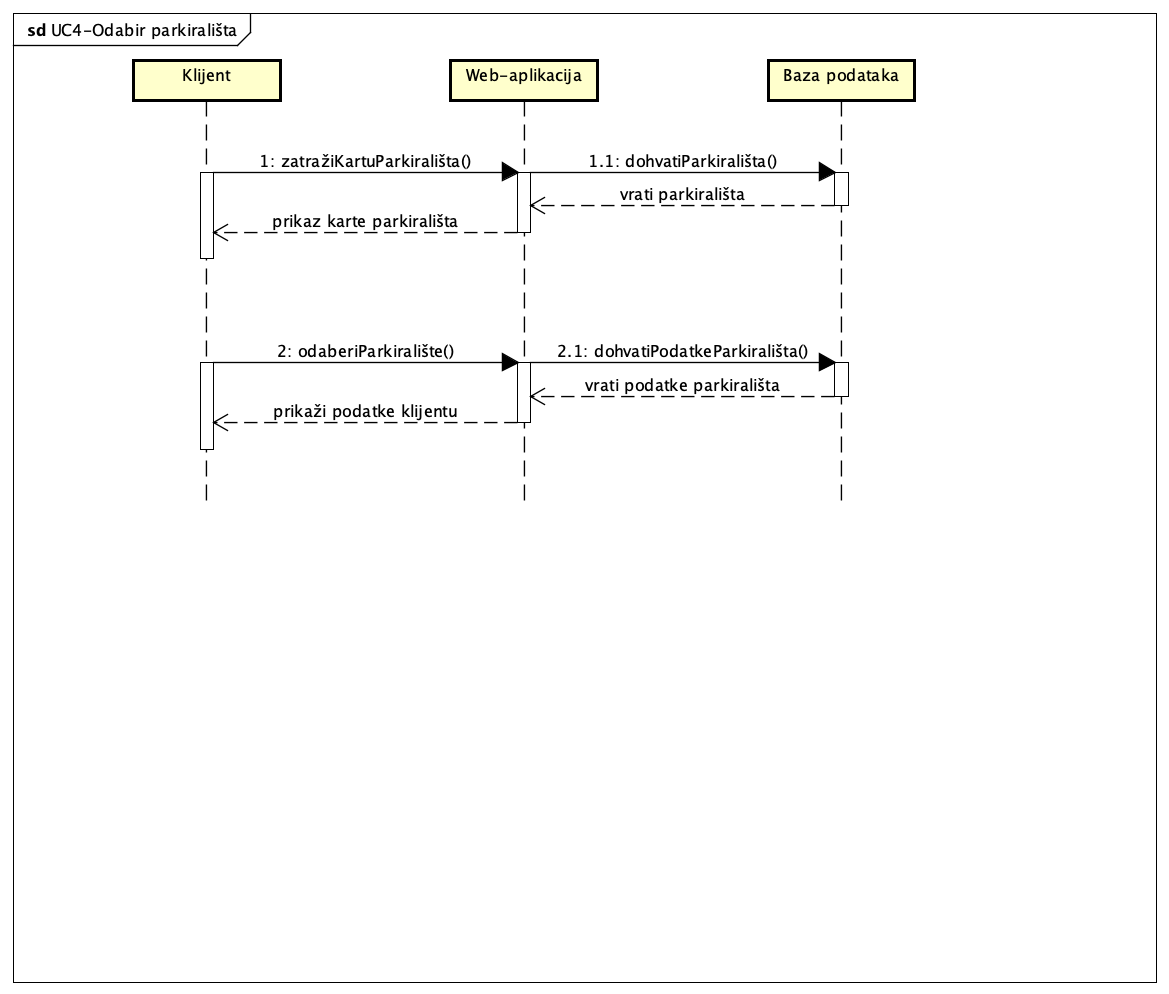
\includegraphics[width=0.7\linewidth]{../../../uc4}
				    	   \caption{Sekvencijski dijagram za UC4}
				        	\label{fig:uc4}
				       \end{figure}
				    
				    
				    
				    
				    
				    
				   \textbf{\textit{Obrazac uporabe UC5 - Rezervacija mjesta}}
				   
				   
				  
				   \textit{Klijent, nakon što je odabrao željeno parkiralište, pristupa informacijama o dostupnim parkirališnim mjestima. Aplikacija mu prikazuje kartu parkirališta s označenim slobodnim i zauzetim mjestima. Tada klijent šalje upit za odabranim mjestom, a aplikacija provjerava raspoloživost tog mjesta. Ukoliko je mjesto slobodno, klijentu se potvrđuje rezervacija, a sustav ažurira informacije o zauzetosti i evidentira rezervaciju.U slučaju da mjesta nisu slobodna, aplikacija obavještava klijenta o nedostupnosti te ga vraća na korak odabira novih mjesta ili termina.}
				   
				   \pagebreak
				   
				   
				   
				   
				    \begin{figure}[hbt!]
				    	\centering
				    	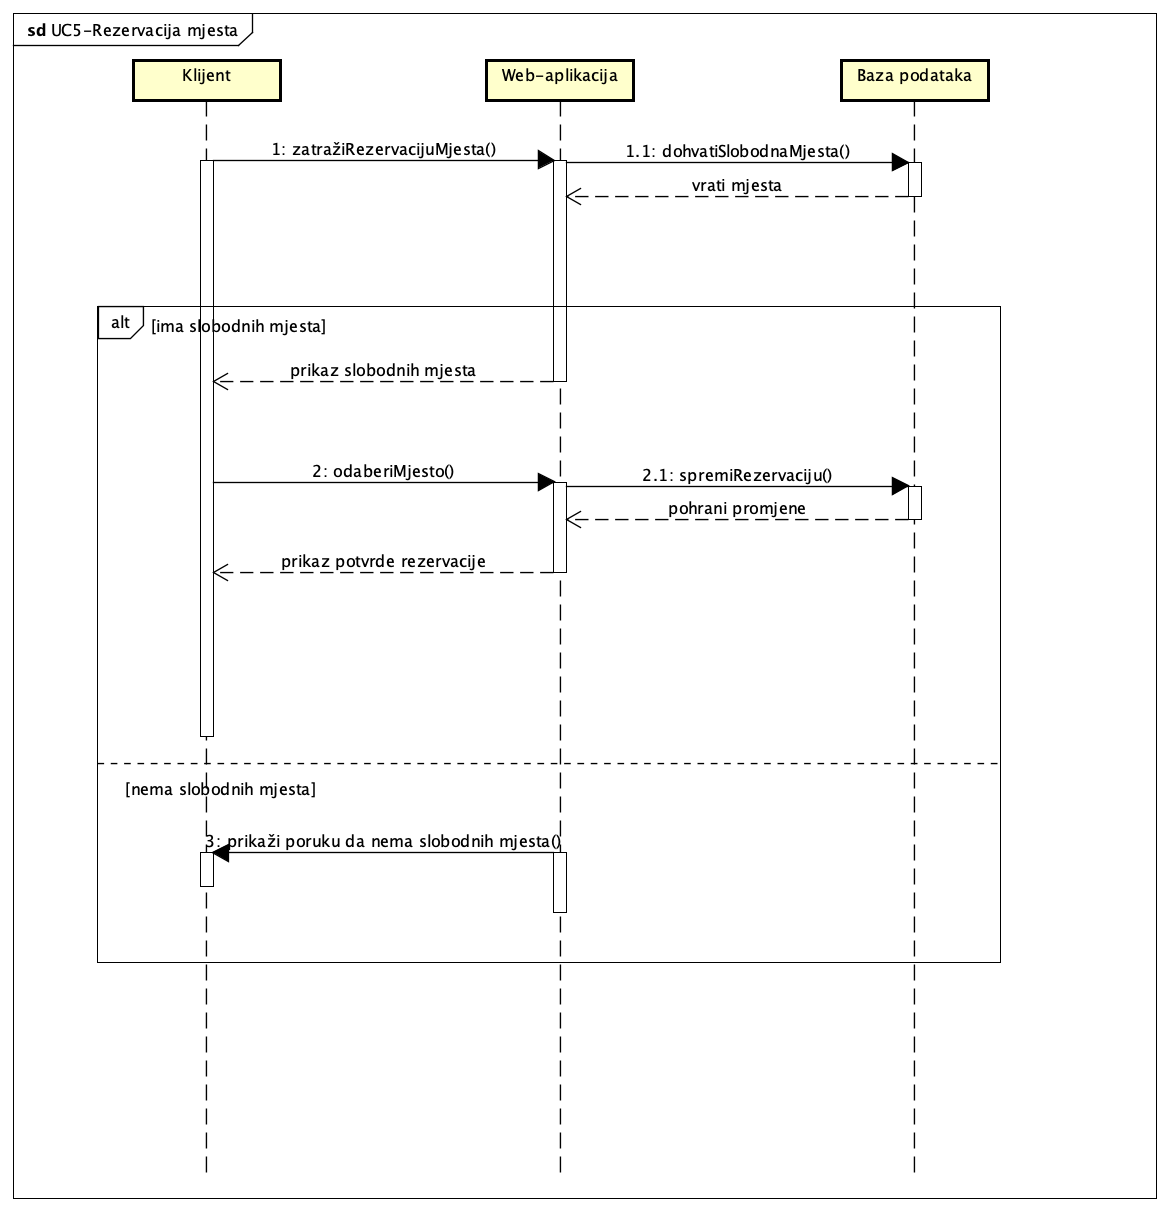
\includegraphics[width=0.7\linewidth]{../../../mjesto}
				    	\caption{Sekvencijski dijagram za UC5}
				    	\label{fig:mjesto}
				    \end{figure}
				    
				    
				    
				    
				    
				    
				    
				    
				    
				    
			     	
				    \textbf{\textit{Obrazac uporabe UC6 - Plaćanje parkirališta}}
				    				
				     \textit{Kada klijent odluči platiti parkiranje, sustav prikazuje opcije plaćanja prilikom rezervacije ili prilikom dolaska na lokaciju parkirališta. Klijent odabire željeni način plaćanja. Ako odabere plaćanje unutar aplikacije, tada aplikacija provjerava stanje novčanika. Rezervacija će se naplatiti ako klijent ima dovoljno sredstava u novčaniku, a u protivnom će mu se prikazati da treba nadoplatit svoj novčanik. Ako se odluči za opciju plaćanja parkinga na parkiralištu, tada će mu aplikacija to prihvatit i potvrdit.}
				     
				     
				     
				      \begin{figure}[hbt!]
				      	\centering
				      	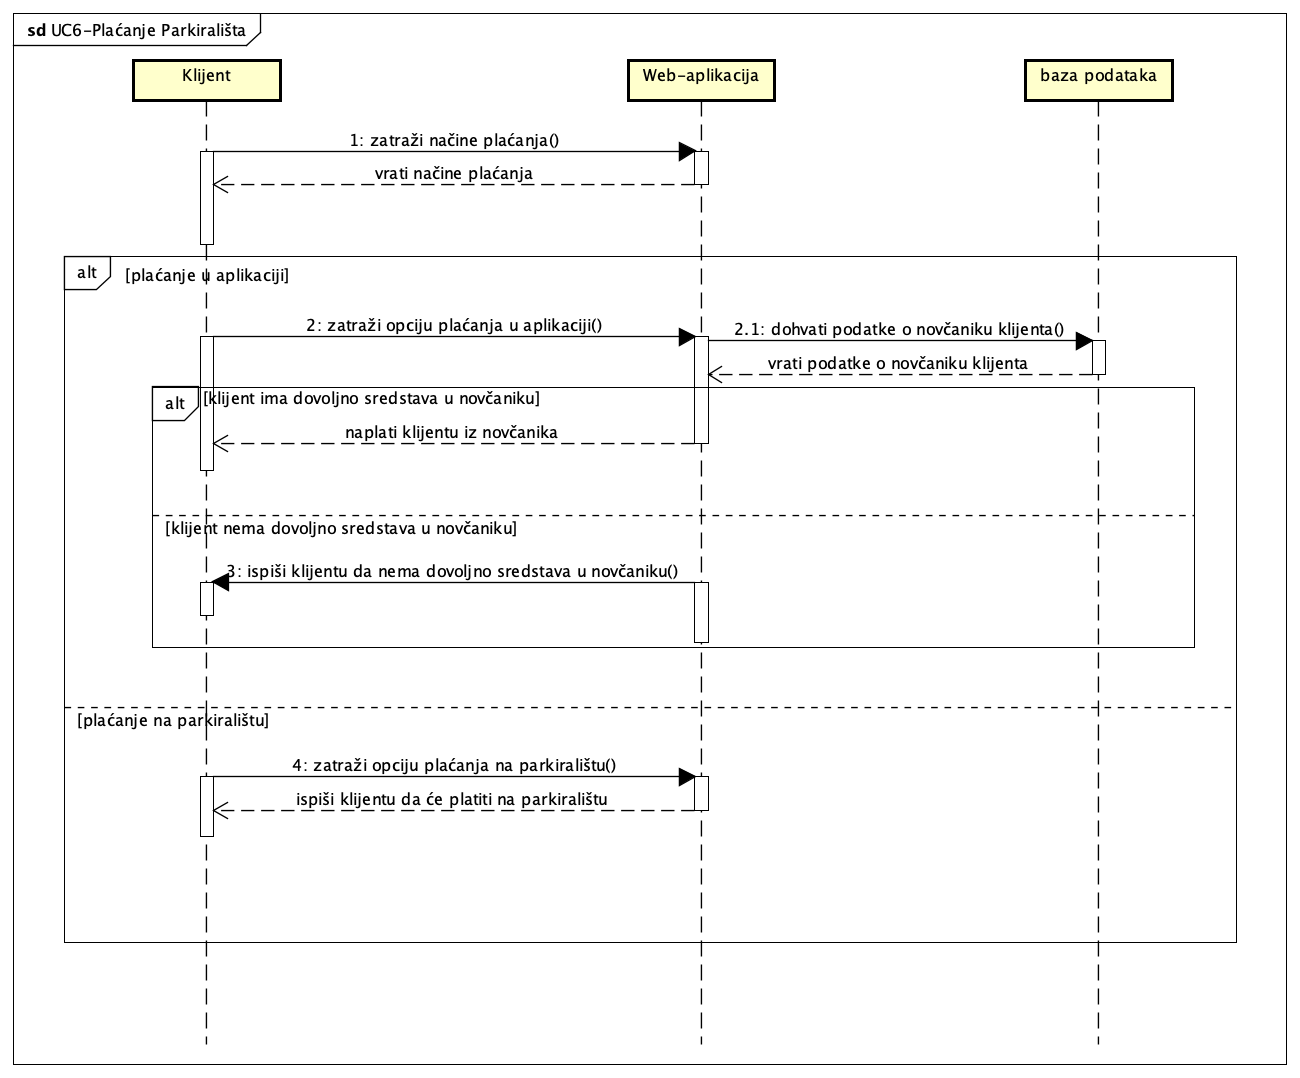
\includegraphics[width=0.7\linewidth]{../../../UC6}
				      	\caption{Sekvencijski dijagram za UC6}
				      	\label{fig:uc6}
				      \end{figure}
				      
				    
				    
				    
		   	\eject
	
		\section{Ostali zahtjevi}
		
			\textbf{\textit{dio 1. revizije}}\\
		 
			 \textit{Nefunkcionalni zahtjevi i zahtjevi domene primjene dopunjuju funkcionalne zahtjeve. Oni opisuju \textbf{kako se sustav treba ponašati} i koja \textbf{ograničenja} treba poštivati (performanse, korisničko iskustvo, pouzdanost, standardi kvalitete, sigurnost...). Primjeri takvih zahtjeva u Vašem projektu mogu biti: podržani jezici korisničkog sučelja, vrijeme odziva, najveći mogući podržani broj korisnika, podržane web/mobilne platforme, razina zaštite (protokoli komunikacije, kriptiranje...)... Svaki takav zahtjev potrebno je navesti u jednoj ili dvije rečenice.}
			 
			 
			 
	